% !TEX root =paper.tex

\section{Preliminaries}
\subsection{Notation}
We write $[n]:=\{1,\dots,n\}$ to denote the set of integers from $1$ to $n$.

For a set $S\subseteq V$, we write 
$$E(S)=\{(u,v)\in E: u,v\in S\}$$ to denote the set of edges in $S$ and we write 
$$\delta(S)=\{(u,v)\in E: |\{u,v\}\cap S|=1\}$$ 
to denote the  set of edges that leave $S$. 

For two {\em disjoint} sets of vertices $A,B\subseteq V$, we write
$$ E(A,B)=\{(u,v)\in E: u\in A, v\in B\}.$$

For a set $A\subseteq E$ and a function $x:E\to\R$ we write
$$ x(A):=\sum_{e\in A} x_e.$$

\hypertarget{tar:crossing}{For two sets $A,B\subseteq V$, we say $A$ {\em crosses} $B$ if all of the following sets are non-empty:
$$ A\cap B, A\smallsetminus B, B\smallsetminus A, \overline{A\cup B}.$$}

\hypertarget{tar:G=(V,E,x)}{We write $G=(V,E,x)$ to denote an (undirected) graph $G$ together with special vertices $u_0,v_0$ and a weight function $x:E\to\R_{\geq 0}$ such that 
$$x(\delta(S))\geq 2, \quad\quad \forall S\subsetneq V: u_0,v_0\notin S.$$}
\hypertarget{tar:nearmincut}{For such a graph, we say a cut $S\subseteq V$ is an {\em $\eta$-near min cut w.r.t., $x$} (or simply $\eta$-near min cut when $x$ is understood) if $x(\delta(S))\leq 2+\eta$.}
Unless otherwise specified, in any statement about a cut $(S,\overline{S})$ in $G$,  we assume $u_0,v_0\not\in S$. 

\subsection{Polyhedral Background}
For any graph $G=(V,E)$,
Edmonds \cite{Edm70} gave the following description for the convex hull of spanning trees of a graph $G=(V,E)$, known as the {\em spanning tree polytope}.
\begin{equation}
\begin{aligned}
& z(E) = |V|-1 & \\
& z(E(S)) \leq |S|-1 &  \forall S\subseteq V\\
& z_e \geq 0 & \hspace{6ex} \forall e\in E.
\end{aligned}
\label{eq:spanningtreelp}
\end{equation}
Edmonds \cite{Edm70} proved that the extreme point solutions of this polytope are the characteristic vectors of the spanning trees of $G$. 



%We formally define tight sets in \cref{subsec:algorithm} but for now assume $S$ is tight if $x(\delta(S))=2$. In the half-integral case this corresponds to $|\delta(S)|=4$.
\begin{fact} \label{fact:sptreepolytope}
Let $x^0$ be a feasible solution of the \ref{eq:tsplp} such that $x^0_{e_0}=1$ with support $E_0=E\cup \{e_0\}$. %Let $E$ be the support of $x$ excluding $e_0$. Then, 
Let $x$ be $x^0$ restricted to $E$; then $x$ is in the spanning tree polytope of $G=(V,E)$. 
\end{fact}
\begin{proof}
%Let $x$ be the restriction of $x$ to $E$.
For any set $S\subseteq V$ such that $u_0,v_0\notin S$, $x(E(S))=\frac{2|S|-x^0(\delta(S))}{2}\leq |S|-1$.
If $u_0\in S, v_0\notin S$, then
$x(E(S)) = \frac{2|S|-1 - (x^0(\delta(S)) -1 )}{2}\leq |S|-1$.
Finally, if $u_0,v_0\in S$, then 
$x(E(S)) = \frac{2|S|-2 - x^0(\delta(S))}{2} \leq |S|-2$.
The claim follows because $x(E)=x^0(E_0)-1=n-1$.
 \end{proof}


Since $c(e_0)=0$, the following fact is immediate.
\begin{fact} \label{fact:expcostT}Let $G=(V,E,x)$ where  $x$ is in the spanning tree polytope. Let $\mu$ be any distribution of spanning trees with marginals $x$, then $\EE{T\sim\mu}{c(T \cup e_{0})}=c(x)$.
 \end{fact}
 
To bound the cost of the min-cost matching on the set $O$ of odd degree vertices of the tree $T$, we use the following characterization of the $O$-join polytope\footnote{The standard name for this is the $T$-join polytope. Because we reserve $T$ to represent our tree, we call this the $O$-join polytope, where $O$ represents the set of odd vertices in the tree.} due to Edmonds and Johnson \cite{EJ73}.
%%%copied from tsp-journal
\begin{proposition}
\label{prop:tjoin}
For any graph $G=(V,E)$, cost function $c: E \to \R_+$, and a set $O\subseteq V$ with an even number of vertices,  the minimum weight of an $O$-join equals the optimum value of the following integral linear program.
\begin{equation}
\begin{aligned}
\min \hspace{4ex} & \cost(y) \\
\st \hspace{3ex} & y(\delta(S)) \geq 1 & \forall S \subseteq V, |S\cap  O| \text{ odd}\\
& y_e \geq 0 & \forall e\in E
\end{aligned}
\label{eq:tjoinlp}
\end{equation}
\end{proposition}

\begin{definition}[Satisfied cuts]\label{def:satisfiedcuts}
\hypertarget{tar:satisfy}{For a set $S\subseteq V$ such that $u_0,v_0\notin S$ and a spanning tree $T\subseteq E$ we say a vector $y:E\to\R_{\geq 0}$ 	satisfies $S$ if one of the following holds:
\begin{itemize}
\item $\delta(S)_T$ is even, or
\item $y(\delta(S))\geq 1$.	
\end{itemize}}
\end{definition}
To analyze our algorithm, we will see that the main challenge is to construct a (random) vector $y$ that satisfies all  cuts and $\E{c(y)}\leq (1/2-\eps)OPT$. 


% \subsection{Maximum entropy distribution}
% We say a distribution $\mu$ over spanning trees is 
%{\em $\lambda$-uniform or maximum entropy} if there are nonnegative
%weights $\lambda: E \rightarrow  \R_+$ such that for any tree $T$,  
%$$ \P{T} \propto \prod_{e \in T} \lambda_e.$$
%
%Given a point $z$ in the spanning tree polytope, for a connected graph $G = (V, E)$, Asadpour et al. \cite{AGMOS17} show that there is an efficient algorithm
%that
%finds non-negative $\lambda_e$'s in a  such a way that for every edge
%$e \in E$ and tree $T$ sampled from $\mu$, $\P{e \in T}$ is
%(approximately) equal to $z_e$.
%
%
%To sample from a distribution on spanning trees, we follow \cite{AGMOS17,OSS11} and 
% sample spanning trees using a distribution
%
%
%We can now briefly explain the main algorithm of \cite{OSS11}: Given a feasible solution $x$ of subtour-LP, define $z=(1-1/n)x$. Then, sample $T$ from a $\lambda$-uniform distribution with marginals $z$ and add a min-cost matching on the odd degree vertices of $T$.

%The crucial aspect of this method of sampling is that the resulting distribution of spanning trees is \textbf{strongly Rayleigh}, which guarantees many strong and useful
%properties beyond negative correlation between the edges of random spanning trees and concentration. For example, Strongly Rayleigh measures~\cite{BBL09} are also
%closed under projection and truncation and conditioning in certain scenarios.

%\subsection{Min-cost Eulerian augmentation}
%\label{sec:Ojoin}
%Once we have sampled a tree (or, as we shall see later, a tree plus an edge), we will be finding the minimum cost Eulerian augmentation. 


\subsection{Structure of Near Minimum Cuts}\label{sec:structure-NMC}

%Here we will review more general properties of near minimum cuts. In the following three lemmas, consider the cuts in any $\con$-connected graph, and call $(A,\overline{A})$ a $(1+\epsilon)$ near minimum cut if $\delta(S) \ge \con(1+\epsilon)$. For generality, we use $|\delta(S)|$ to denote the capacity of the cut. 
%In the following three lemmas assume $G=(V,E)$ and $x:E\to\R_{\geq 0}$ such that for every $S\subsetneq V$, $x(\delta(S))\geq 2$.

%This first lemma is proved in :
\begin{lemma}[\cite{OSS11}]\label{lem:cutdecrement}
For $G=(V,E,x)$, let $A,B\subsetneq V$ be two crossing $\eps_A, \eps_B$ near min cuts respectively. Then,
$A\cap B, A\cup B, A\smallsetminus B, B\smallsetminus A$ are $\eps_A+\eps_B$ near min cuts.
\end{lemma}
\begin{proof}
We prove the lemma only for $A\cap B$; the rest of the cases can be proved similarly.
%Since the cut function $|\delta(.)|$ is a submodular function we have
By submodularity,
$$ x(\delta(A\cap B)) + x(\delta(A\cup B)) \leq x(\delta(A)) + x(\delta(B)) \leq 4+\eps_A+\eps_B.$$
Since $x(\delta(A\cup B))\geq 2$, we have $x(\delta(A\cap B))\leq 2+\epsilon_A+\eps_B$, as desired.
\end{proof}

The following lemma is proved in \cite{Ben97}:
\begin{lemma}[{\cite[Lem 5.3.5]{Ben97}}]
\label{lem:nmcuts_largeedges}
For $G=(V,E,x)$, let $A,B\subsetneq V$ be two crossing $\eps$-near minimum cuts. %such that %$x(\delta(A)),x(\delta(B)) \le 2+\epsilon$. Then 
Then, $$x(E(A\cap B, A\setminus B)),x(E(A\cap B, B\setminus A)), x(E(\overline{A\cup B}, A\setminus B)), x(E( \overline{A\cup B}, B\setminus A)) \geq (1-\epsilon/2).$$
%Let $(A,\overline{A})$ and $(B,\overline{B})$ be two crossing $(1+\epsilon)$ near minimum cuts of $G$. Then $|E(A\cap B, A\setminus B)| \geq (1-\epsilon)\frac{\con}{2}$.
\end{lemma}
%Note that by symmetry it can be derived from the above lemma that
%%\begin{equation*}
%\begin{eqnarray*}
% \geq (1-\epsilon)\frac{\con}{2}\\
%  \geq (1-\epsilon)\frac{\con}{2} \\
%  \geq (1-\epsilon)\frac{\con}{2}
%\end{eqnarray*}
%
%We show one additional lemma:
\begin{lemma}
\label{lem:shared-edges}
For $G=(V,E,x)$, let $A,B\subsetneq V$ be two $\eps$ near min cuts  such that $A \subsetneq B$. Then 
$$x(\delta(A) \cap \delta(B)) = x(E(A,\overline{B}))\le 1 + \eps, \text{ and }$$
$$x(\delta(A)\smallsetminus \delta(B))\geq 1-\eps/2. $$
%Let $S,T$ be two sets such that $S \subsetneq T$ and $|\delta(S)|,|\delta(T))| \le \con(1+\epsilon)$. Then 
%$$|\delta(S) \cap \delta(T)| = |E(S,\overline{T})|\le \bigg(\frac{1}{2}+\epsilon\bigg)\con.$$
\end{lemma}
\begin{proof}
Notice
\begin{align*}&2+\epsilon \ge x(\delta(A)) = x(E(A,B \smallsetminus A)) + x(E(A,\overline{B}))\\
&2+\epsilon \ge x(\delta(B)) = x(E(B \smallsetminus A,\overline{B})) + x(E(A,\overline{B}))
\end{align*}
Summing these up, we get
$$2x(E(A,\overline{B})) + x(E(A,B \smallsetminus A)) + x(E(B \smallsetminus A, \overline{B})) = 2x(E(A,\overline{B}))+x(\delta(B\smallsetminus A)) \le 4+2\eps.$$
Since $B \smallsetminus A$ is non-empty,
	$x(\delta(B\smallsetminus A)) \ge 2$,
which implies the first inequality.
To see the second one, let $C=B\smallsetminus A$ and note
$$ 4\leq x(\delta(A))+x(\delta(C)) = 2 x(E(A,C)) + x(\delta(B))\leq 2 x(E(A,C))+ 2+\eps$$
which implies $x(E(A,C))\geq 1-\eps/2$.
\end{proof}

%For the benefit of the reader, we rewrite these lemmas using notation consistent with the rest of the paper and set $\con = 2$ as is the case in the support graph of $x$:

%\begin{lemma}
%\label{lem:cutdecrement}
%Let $A$ and $B$ be two crossing cuts such that $x(\delta(A)) \le 2+\epsilon$. Then,
%$$ \max\{ x(\delta(A\cap B))|, x(\delta(A\cup B)), x(\delta(A\smallsetminus B)), x(\delta(B\smallsetminus A))\}
%\leq  x(\delta(B)) + \eps.$$
%%Moreover, $\delta(B\cap A) + \delta(B\setminus) \leq \delta(B)+$.
%\end{lemma}
%\begin{lemma}
%\label{lem:nmcuts_largeedges}
%Let $A$ and $B$ be two crossing near minimum cuts such that $x(\delta(A)),x(\delta(B)) \le 2+\epsilon$. Then $|E(A\cap B, A\setminus B)| \geq (1-\epsilon/2)$.
%\end{lemma}
%\begin{lemma}\label{lem:shared-edges}
%Let $A,B$ be two cuts such that $A \subsetneq B$ and $x(\delta(A))),x(\delta(B))) \le 2+\epsilon$. Then 
%$$x(\delta(A) \cap \delta(B)) = x(E(S,\overline{B}))\le 1 + \eps.$$
%\end{lemma} 

%\Nathan{I'm not sure this next lemma is needed, it's fairly obvious and only cited once. Do we use it implicitly elsewhere?}




\def\ber{\textup{Ber}}
\def\bin{\textup{Bin}}
\def\Poi{\textup{Poi}}

\def\ber{\textup{Ber}}
\def\bin{\textup{Bin}}
\def\Poi{\textup{Poi}}

\subsection{Strongly Rayleigh Distributions and $\lambda$-uniform Spanning Tree Distributions}
\label{sec:SRdistns}
%We say a polynomial $p\in \R_{\geq 0}[z_1,\dots,z_n]$ is {\em real stable} if it has no roots in the upper-half complex plane, i.e., $p(z)\neq 0$ whenever $\Im(z_i)>0$ for all $i$.
%We write $[n]:=\{1,\dots,n\}$.
%For a probability distribution $\mu:2^{[n]}\to \R_{\geq 0}$, $g_\mu:=\sum_{S\subseteq [n]} \mu(S) z^S$ is called the generating polynomial of $\mu$ where $z^S=\prod_{i\in S} z_i$.
%We say $\mu$ is {\em strongly Rayleigh} if $g_\mu$ is a real stable polynomial.
Let $\cB_E$ be the set of all probability measures on the Boolean algebra $2^E$. 
Let $\mu\in\cB_E$. The generating polynomial $g_\mu: \R[\{z_{e}\}_{e\in E}]$ of $\mu$ is defined as follows:
$$ g_\mu(z):=\sum_S \mu(S) \prod_{e\in S} z_e.$$
\hypertarget{tar:SR}{We say $\mu$ is a strongly Rayleigh distribution if $g_\mu\neq 0$ over all $\{y_e\}_{e\in E} \in \mathbb{C}^E$ where $\text{Im}(z_e)>0$ for all $e\in E$. We say $\mu$ is $d$-homogenous if for any $\lambda \in \R$, $g_\mu(\lambda {\bf z}) = \lambda^d g_\mu({\bf z})$.}
Strongly Rayleigh (SR) distributions were defined in \cite{BBL09} where it was shown any $\lambda$-uniform spanning tree distribution is strongly Rayleigh. In this subsection we recall several properties of SR distributions proved in \cite{BBL09,OSS11} which will be useful to us.


\paragraph{Closure Operations of SR Distributions.}
SR distributions are closed under the following operations.

\begin{itemize}
	\item {\bf Projection.} For any $\mu\in \cB_E$, and any $F\subseteq E$, the projection of $\mu$ onto $F$ is the measure $\mu_F$
	where for any $A\subseteq F$,
	$$ \mu_F(A)=\sum_{S: S\cap F=A} \mu(S).$$
	\item {\bf Conditioning.} For any $e\in E$, $\{\mu | e \text{ out}\}$ and $\{\mu | e \text{ in}\}$.
	\item {\bf Truncation.} For any integer $k\geq 0$ and $\mu\in \cB_E$, truncation of $\mu$ to $k$, is the measure $\mu_k$ where for any $A\subseteq E$,
$$ \mu_k(A)=\begin{cases} \frac{\mu(A)}{\sum_{S:|S|=k} \mu(S)} & \text{if } |A|=k\\ 0 & \text{otherwise.}\end{cases}$$
	\item {\bf Product.} For any two disjoint sets $E,F$, and $\mu_E\in \cB_E,\mu_F\in\cB_F$ the product measure $\mu_{E\times F}$ is the measure where for any $A\subseteq E,B\subseteq F$, $\mu_{E\times F}(A\cup B)=\mu_E(A)\mu_F(B)$.
\end{itemize}
Throughout this paper we will repeatedly apply the above operations. 
We  remark that SR distributions are {\em not} necessarily closed under truncation of a subset, i.e., if we require exactly $k$ elements from $F\subsetneq E$.


%To contrast the above definition with random spanning trees we also explain closure properties of
%Note that
Since $\lambda$-uniform spanning tree distributions are special classes of SR distributions, if we perform any of the above operations on a $\lambda$-uniform spanning tree distribution $\mu$ we get another SR distribution. Below, we see that by performing  the following particular operations we still have a $\lambda$-uniform spanning tree distribution (perhaps with a different $\lambda$). 
\paragraph{Closure Operations of $\lambda$-uniform Spanning Tree Distributions}
For $G=(V,E)$, a spanning tree distribution $\mu\in \cB_E$, and $T \sim \mu$, we have:
\begin{itemize}
	\item {\bf Conditioning}. For any $e\in E$, $\{\mu \mid e \not\in T\}, \{\mu \mid e \in T\}$. 
	\item {\bf Tree Conditioning}. For $S\subseteq V$, $\{\mu \mid |E(S) \cap T| = |S|-1\}$, i.e. $T$ restricted to $S$ is a tree. We will often just write $S\text{ is a tree}$ to denote such an event.
\end{itemize}
Note that arbitrary spanning tree distributions are not necessarily closed under truncation and projection. 
We remark that SR measures are also closed under an analogue of tree conditioning, i.e., for a set $F\subseteq E$, let $k=\max_{S\in\text{supp }\mu} |S\cap F|$. Then, $\{\mu \mid |S\cap F|=k\}$ is SR. But if $\mu$ is a spanning tree distribution we get an extra {\em independence} property. The following independence is crucial to several of our proofs.
\begin{fact}
\label{fact:treeIndep}
For a graph $G = (V,E)$, and a vector $\lambda (G): E\rightarrow \R _{\ge 0}$, let $\mu_{\lambda(G)}$ be the corresponding $\lambda$-uniform spanning tree distribution.
Then for any $S\subsetneq V$, 
	$$\{\mu_{\lambda(G)} \mid S\text{ is a tree}\} = \mu_{\lambda(G[S])} \times  \mu_{\lambda(G/S)}.$$ 
\end{fact}
\begin{proof}
	Intuitively, this holds because in the max entropy distribution (recall a $\lambda$-uniform distribution maximizes entropy subject to matching the marginals of $x$), conditioned on $S$ being a tree, any tree chosen inside $S$ can be composed with any tree chosen on $G/S$ to obtain a spanning tree on $G$. So, to maximize the entropy these trees should be chosen independently. %follows by subadditivity of entropy
	More formally for any $T_1 \in G[S]$ and $T_2 \in G/S$, 
	\begin{align*}
	\P{T=T_1\cup T_2 \mid S\text{ is a tree}} &= \frac{\lambda^{T_1}\lambda^{T_2}}{\sum_{T'_1 \in G[S],T'_2 \in G/S} \lambda^{T'_1}\lambda^{T'_2}} \\ 
	&= \frac{\lambda^{T_1}}{\sum_{T'_1 \in G[S]} \lambda^{T'_1}} \cdot \frac{\lambda^{T_2}}{\sum_{T'_2 \in G/S} \lambda^{T'_2}} \\
	&= \PP{T'_1 \sim G[S]}{T'_1 = T_1}\PP{T'_2 \sim G/S}{T'_2 = T_2},
	\end{align*}
giving independence.
\end{proof}



\paragraph{Negative Dependence Properties.}
An {\em upward event}, ${\cal A}$, on $2^E$ is a collection of subsets of $E$ that is closed  under upward containment, i.e. if $A\in{\cal A}$ and $A\subseteq B\subseteq E$, then $B\in{\cal A}$. Similarly, a {\em downward event} is closed  under downward  containment.
An {\em increasing function} $f:2^E\rightarrow \R$, is a function where for any $A\subseteq B\subseteq E$, we have $f(A)\leq f(B)$. We also say $f:2^E\to\R$ is a {\em decreasing function} if $-f$ is an increasing function.
So, an indicator of an upward event is an increasing function.
%Any (non-identically zero) non-negative increasing function $f$ on $2^E$, may be written as $f:=\sum_{i=1}^k \alpha_i \chi_{\
For example, if $E$ is the set of edges of a graph $G$, then the existence of a Hamiltonian cycle is an increasing function, and the $3$-colorability of $G$ is a decreasing function.

\begin{definition}[Negative Association]
\label{def:negativeassociation}
A measure $\mu \in {\cal B}_E$ is {\em negatively associated} if 
for any increasing functions $f,g: 2^E\to \R$, that depend on {\em disjoint} sets of edges,
$$ \EE{\mu}{f}\cdot \EE{\mu}{g} \geq  \EE{\mu}{f\cdot g} $$
%for any increasing functions F, G on $2^E$ that depend on disjoint sets of elements.
\end{definition}
%Feder and Mihail \cite{FM92} proved that  uniform measures on balanced matroids (and in particular
% $\lambda$-uniform spanning tree distributions) are negative associated.
It is shown in \cite{BBL09,FM92}  that strongly Rayleigh measures
are negatively associated. 

\paragraph{Stochastic Dominance.}
%First, we recall the {\em stochastic dominance} property.
For two measures $\mu,\nu:2^{E}\to\R_{\geq 0}$, we say $\mu \preceq \nu$ if there exists a {\em coupling} $\rho: 2^{E}\times 2^{E} \to\R_{\geq 0}$ such that 
\begin{eqnarray*}
	\sum_B \rho(A,B)&=&\mu(A), \forall A\in 2^{E},\\
	\sum_A \rho(A,B)&=& \nu(B), \forall B\in 2^{E},
\end{eqnarray*} 
and for all $A,B$ such that $\rho(A,B)>0$ we have $A\subseteq B$ (coordinate-wise).

\begin{theorem}[\cite{BBL09}]
\label{thm:stochDom}
	If $\mu$ is strongly Rayleigh and $\mu_k,\mu_{k+1}$ are well-defined, then $\mu_k \preceq \mu_{k+1}$.
\end{theorem}
Note that in the above particular case the coupling $\rho$ satisfies the following: For any $A,B\subseteq E$ where $\rho(A,B)>0$, $B\supseteq A$ and $|B\smallsetminus A|=1$, i.e., $B$ has exactly one more element.


Let $\mu$ be a strongly Rayleigh measure on edges of $G$. Recall that for a set $A\subseteq E$, we write $A_T=|A\cap T|$ to denote the random variable indicating the number of edges in $A$ chosen in a random sample $T$ of $\mu$. The following facts immediately follow from the negative association and stochastic dominance properties. We will use these facts repeatedly in this paper. 
%\begin{theorem}[{\cite{BBL09}}]
%\label{thm:rayleigh_negativeassocation}
%Strongly Rayleigh measures are negatively associated.
%\end{theorem}

\begin{fact}[{\cite[Theorems 4.8, 4.19]{BBL09}}]
\label{fact:updown}
Let $\mu$ be any SR distribution on $E$, then
for any $F\subset E$, and any integer $k$
\begin{enumerate}
\item (Negative Association) If $e\notin F$, then $\PP{\mu}{e \big| F_T \geq k} \leq \PP{\mu}{e}$ and 
$\PP{\mu}{e | F_T \leq k} \geq \PP{\mu}{e} $
\item (Stochastic Dominance) If $e\in F$, then $\PP{\mu}{e | F_T \geq k} \geq \PP{\mu}{e}$ and $\PP{\mu}{e | F_T\leq k} \leq \PP{\mu}{e}$.
\end{enumerate}
\end{fact}

The following fact is a direct consequence of the above, see e.g. Corollary 6.10 of \cite{OSS11}.
\begin{fact}
\label{fact:e1}
Let $\mu$ be a homogenous SR distribution on $E$. Then,
%For any set $S \subset V$ and $A\subseteq E$,
\begin{itemize}
\item (Negative association with homogeneity) For any $A\subseteq E$, and  any $B\subseteq \overline{A}$ 
\begin{equation} \EE{\mu}{ B_T | A_T = 0} \leq \EE{\mu}{B_T} + \EE{\mu}{A_T} 
%\text{ and } \EE{\mu}{A'_T | A_T = 0} 
\label{fact:e0}
\end{equation}	
\item Suppose that $\mu$ is a spanning tree distribution. For  $S\subseteq V$, let $q:=|S|-1-\EE{\mu}{E(S)_T}$.  For any $A\subseteq E(S), B\subseteq \overline{E(S)}$,
\begin{align}
&\EE{\mu}{B_T}  - q \le \EE{\mu}{ B_T | S\text{ is a tree}} \le \EE{\mu}{B_T}\tag{Negative association and homogeneity}\\
 &\EE{\mu}{A_T}
 \leq \EE{\mu}{A_T | S\text{ is a tree}} \leq \EE{\mu}{A_T}+q
\tag{Stochastic dominance and tree}
\end{align}
\end{itemize}
\end{fact}
%\begin{lemma} \label{lem:correlation}
%Let $S = \{e_1, \ldots, e_k\}$ be a set of  $k$ edges and suppose that $e \not\in S$. 
%Then there are $k-1$ edges in $S$ such that for each edge $e_i$ among these $k-1$
%$$0.25  \le \P{e_i \in T | e \in T} \le 0.5.$$
%\end{lemma}
%
%\begin{proof}
%By \cref{fact:e1}, $\P{e_i | e\in T} \leq 0.5$ for all $e_i$.
%Suppose that (after renaming) $\P{e_1 | e\in T}$ and $\P{e_2 | e\in T}$ are the smallest among all $1\leq i\leq k$. Observe that  by \cref{fact:e1} $\E{X_{e_1}+X_{e_2} | e\in T}\geq 0.5$. Therefore, the bigger one is at least $0.25$.
%\end{proof}



\paragraph{Rank Sequence.}

The {\em rank sequence} of $\mu$ is the sequence
$$\P{|S|=0}, \P{|S|=1}, \ldots,\P{|S|=m},$$
where $S\sim\mu$.
Let $g_\mu({\bf z})$ be the generating polynomial of $\mu$.
The {\em diagonal specialization} of $\mu$ is the univariate polynomial 
$$\bar{g}_\mu(z):=g_\mu(z,z,\dots,z). $$ Observe that $\bar{g}(.)$ is the generating polynomial of the rank sequence of $\mu$. It follows that if $\mu$ is SR then $\bar{g_\mu}$ is real rooted.
%If $\bar{g}(c)=0$ for $c\in \mathbb{C}$, then $g(c,c,\dots,c)=0$. So,  if $g(.)$ is a real stable polynomial then so is $\bar{g}$. Since a univariate polynomial with real coefficients is stable if and only if all of its roots are real, $\bar{g}(.)$ is a polynomial with real roots.



It is not hard to see that the rank sequence of $\mu$ corresponds to sum of independent Bernoullis iff $\bar{g_\mu}$ is real rooted. It follows that the rank sequence of an SR distributions has the law of a sum of independent Bernoullis. As a consequence, 
it follows  (see \cite{HLP52,Dor64,BBL09})
that the rank sequence of any strongly Rayleigh measure is  log concave (see below for the definition), unimodal, and its mode differs from the mean by less than 1.
\begin{definition}[Log-concavity {\cite[Definition 2.8]{BBL09}}]
A real sequence $\{a_k\}^m_{k=0}$ is log-concave if $a^2_k \geq a_{k-1}\cdot a_{k+1}$ for all $1 \leq k\leq m-1$, and it is said to have no internal zeros if the indices of its non-zero terms form an interval (of non-negative integers). 
\end{definition}


\subsection{Sum of Bernoullis}
In this section, we collect a number of properties of sums of Bernoulli random variables.

\begin{definition}[Bernoulli Sum Random Variable]\label{def:BS}\hypertarget{tar:BS}{
We say $BS(q)$ is a {\em Bernoulli-Sum} random variable if it has the law of a sum  of independent Bernoulli random variables, say $B_1 + B_2 + \ldots +B_n$  for some $n\ge 1$, with $\E{B_1+ \dots +B_n} = q$. }
\end{definition}

We start with the following theorem of Hoeffding.
\begin{theorem}[{\cite[Corollary 2.1]{Hoe56}}]\label{thm:hoeffding}
Let $g:\{0,1,\dots,n\}\to \R$ and $0\leq q\leq n$ for some integer $n\geq 0$.  Let $B_1,\dots,B_n$ be $n$ independent Bernoulli random variables with success probabilities $p_1,\dots,p_n$, where $\sum_{i=1}^n p_n = q$ that minimizes (or maximizes)
$$ \E{g(B_1+\dots+B_n)}$$
over all such distributions. Then,  $p_1,\dots,p_n\in\{0,x,1\}$ for some $0<x<1$. In particular, if only $m$ of $p_i$'s are nonzero and $\ell$ of $p_i$'s are 1, then the remaining $m-\ell$ are $\frac{q-\ell}{m-\ell}$.
\end{theorem}

\begin{fact} \label{fact:evensum} Let $B_1, \ldots, B_n$ be independent Bernoulli random variables each with expectation $0\le p\le 1$.
Then $$\P{\sum_i B_i \text{ even}} = \frac{1}{2} (1+ (1-2p)^n)$$
%So, in the case that $pn\geq 1$, this is at most $1/2(1+e^{-2}) \leq 0.57$
\end{fact}
\begin{proof}
Note that
$$
 (p+(1-p))^n = \sum_{k=0}^n p^k (1-p)^{n-k} {n\choose k}\quad\text{ and }\quad
 ((1-p)-p)^n = \sum_{k=0}^n (-p)^k (1-p)^{n-k} {n\choose k}	
$$
Summing them up we get,
$$ 1+ (1-2p)^n = \sum_{0\leq k\leq n, k\text{ even}} 2p^k (1-p)^{n-k} {n\choose k}.$$
\end{proof}

\begin{corollary}\label{cor:bernoullisumeven}
Given a $BS(q)$ random variable with $0 < q \le 1.2$,  then
$$ \P{BS(q) \text{ even}} \leq \frac12(1+e^{-2q})$$
\end{corollary}
\begin{proof}
First, if $q\leq 1$, then by Hoeffding's theorem we can write $BS(q)$ as sum of $n$ Bernoullis with success probability $p=q/n$. If $n=1$, then the statement obviously holds. Otherwise, by the previous fact, we have (for some $n$),
 $$\P{BS(q) \text{ even} } \leq \frac12 (1+(1-2p)^n)) \leq \frac12(1+e^{-2q})$$
 where we used that $|1-2p|\leq e^{-2p}$ for $p\leq 1/2$.
 
So, now assume $q>1$.
Write $BS(q)$ as the sum of $n$ Bernoullis, each with success probabilities $1$ or $p$. First assume we 0have no ones. 
Then, either we only have two non-zero Bernoullis with success probability $q/2$ in which case $\P{BS(q)\text{ even}}\leq 0.6^2 + 0.4^2$ and we are done.
Otherwise, $n\geq 3$ so $p\leq 1/2$ and similar to the previous case we get $\P{BS(q) \text{ even}} \leq \frac12(1+e^{-2q})$.

Finally, if $q>1$ and one of the Bernoullis is always $1$, i.e. $BS(q) = BS(q-1)+1$, then we get
$$\P{BS(q)\text{ even}} = \P{BS(q-1) \text{ odd}} = \frac12(1-(1-2p)^{n-1}) \le 1/2$$
%\leq \frac12(1-e^{-4(q-1)})\leq 0.3$$
%where we used that $1-x\geq e^{-2x}$ for $0\leq x\leq 0.2$.
where we used that $p \le 0.5$ (since $q \le 1.2$).
\end{proof}

%\begin{corollary}
%	Given a $BS(q)$ random variable with $\eps \le q \le 1-\eps$, 
%	$$\min \{\P{BS(q) \text{ even}}, \P{BS(q)\text{ odd}}\} \ge ??$$
%\end{corollary}
%\begin{proof}
%Using ?? and fixing $p=q/n$ for some $n$ by Hoeffding,
%	$$\P{BS(q) \text{ even}} = \frac{1}{2}(1+(1-2p)^n)$$
%If $n=1$, then the minimum probability is $\epsilon$. Otherwise, $n \ge 2$ so $\frac{1}{2}(1+(1-2p)^n)$ is a 
%\end{proof}


\begin{lemma}\label{lem:logconcaveexpecation}
Let $p_0,\dots,p_n$ be a log-concave sequence. If for some $i$, $\gamma p_i \geq p_{i+1}$ for some $\gamma<1$, then,
\begin{align*} 
& \sum_{j=k}^n p_j \leq \frac{p_k}{1-\gamma}, \quad \forall k\geq i\\
& \sum_{j=i+1}^n  p_j\cdot j  \leq \frac{p_{i+1}}{1-\gamma} \left(i+1 + \frac\gamma{1-\gamma}\right).	
\end{align*}
\end{lemma}
\begin{proof}
Since we have a log-concave sequence we can write
\begin{equation}\label{eq:logconcaveseq} \frac{1}{\gamma} \leq \frac{p_i}{p_{i+1}}  \leq \frac{p_{i+1}}{p_{i+2}} \leq \dots 	
\end{equation}
Since all of the above ratios are at least $1/\gamma$, for all $l\geq 1$ we can write
$$  p_{i+l} \leq \gamma^{l-1} p_{i+1}\leq \gamma^l p_i.$$
Therefore, the first statement is immediate and the second one follows,
$$ \sum_{j=i+1}^ n p_j j \leq \sum_{l=0}^\infty \gamma^l p_{i+1} (i+l+1) = p_{i+1} \left(\frac{i+1}{1-\gamma} + \frac\gamma{(1-\gamma)^2}\right)$$
\end{proof}

\begin{corollary}\label{cor:logconcaveexpecation}
	Let $X$ be a $BS(q)$ random variable such that $\P{X=k}\geq 1-\eps$ for some integer $k\geq 1$, $\eps<1/10$.
	Then, $k(1-\eps)\leq q\leq k(1+\eps)+3\eps$.
\end{corollary}
\begin{proof}
	The left inequality simply follows since $X\geq 0$. 	Since $\P{X=k+1}\leq \eps$, we can apply \cref{lem:logconcaveexpecation}  with $\gamma=\eps/(1-\eps)$ to get 
%	$$\E{X | X\geq k+1}\P{X\geq k+1}\leq \frac{\eps}{1-\eps}\left(k+1+\frac{\eps}{1-\eps}\right)$$
%	\anna{Shouldn't this be
	$$\E{X | X\geq k+1}\P{X\geq k+1}\leq \frac{\eps(1-\eps)}{1-2\eps}\left(k+1+\frac{\eps}{1-2\eps}\right)$$
	Therefore,
	$$ q=\E{X}\leq k(1-\eps)+\frac{\eps(1-\eps)}{1-2\eps}(k+1+\frac{\eps}{1-2\eps})\leq k(1+\eps)+3\eps$$
	as desired.
\end{proof}


\begin{fact}\label{fact:1-pm^m}
For  integers $k<t$ and $k-1\leq p\leq k$, 
$$\prod_{i=1}^{k-1} (1-i/t) (1-p/t)^{t-k}\geq e^{-p}.$$
\end{fact}
\begin{proof}
We show that the LHS is a decreasing function of $t$. Since $\ln$ is monotone, it is enough to show 
\begin{align*} 0\geq \partial_t  \ln (\text{LHS}) &= \partial_t \left(\sum_{i=1}^{k-1} \ln(1-i/t) + (t-k)\ln(1-p/t)\right)\\
	&= \frac{1}{t^2}\sum_{i=1}^{k-1} \frac{1}{\frac1{i} - \frac{1}{t}} + \ln(1-p/t) + \frac{(t-k)p}{t(t-p)} 
\end{align*}
Using $\sum_{i=1}^{k-2} \frac{1}{t^2/i-t}\leq \int_{0}^{k-1} \frac{dx}{t^2/x - t}=-(k-1)/t -\ln(1-(k-1)/t)$
it is enough to show
\begin{align*}
0&\geq 	-\frac{k-1}{t} - \ln (1-\frac{k-1}{t}) + \ln(1-p/t) + \frac{(t-k)p}{t(t-p)} + \frac{1}{t^2(\frac1{k-1} - \frac1t)}\\
&= \ln\frac{t-p}{t-k+1} + \frac{p-k}{t-p}+\frac{1}{t}+\frac{k-1}{t(t-k+1)}
\end{align*}
Rearranging, it is equivalent to show
\begin{align*}
\ln (1+\frac{p-k+1}{t-p})	\geq \frac{p-k}{t-p} + \frac{1}{t-k+1}
\end{align*}
Since $p>k-1$, using taylor series of $\ln$, to prove the above it is enough to show
$$ \frac{p-k+1}{t-p} - \frac{(p-k+1)^2}{2(t-p)^2} \geq \frac{p-k}{t-p} + \frac{1}{t-k+1}.$$
This is equivalent to show
$$ \frac{p-k+1}{(t-p)(t-k+1)} \geq \frac{(p-k+1)^2}{2(t-p)^2} \Leftrightarrow \frac{1}{t-k+1} \geq \frac{p-k+1}{2(t-p)} $$
Finally the latter holds because $(t-k+1)(p-k+1)\leq (t-k+1)\leq 2(t-p)$ where we use $t\geq k+1$ and $p\leq k$.
%To see this note that $(1-p/t)^{t-p}$ is a decreasing function of $t$ for $t\geq p$, so it is minimized at $t=\infty$.
%This is because 
%$$\partial_t \left(1-\frac{p}{t}\right)^{t-p} = \left(1-\frac{p}{t}\right)^{t-p}\left(\ln(1-p/t)+\frac{p(t-p)}{t^2(1-p/t)}\right)=\left(1-\frac{p}{t}\right)^{t-p}(\ln (1-p/t)+p/t)$$ 
%but the RHS is non-positive for $t\ge p$.
\end{proof}

Let $\Poi(p,k) = e^{-p}p^k/k!$  be the probability that a Poisson random variable with rate $p$ is exactly $k$; similarly, define $\Poi(p,\leq k),\Poi(p,\geq k)$ as the probability that a Poisson with rate $p$ is at most $k$ or at least $k$.
\begin{lemma}%[\cite{OSS11}]
\label{thm:rayleigh_expectconstprob}
Let $X$ be a Bernoulli sum $BS(p)$ for some $n$. 
 For any integer $k\geq 0$ such that $k-1<p<k+1$, the following holds true
$$\P{X=k} \geq \min_{0\leq\ell \leq p,k} \Poi(p-\ell,k-\ell) \left(1-\frac{p-\ell}{k-\ell+1}\right)^{(p-k)_+}$$
where the minimum is over all nonnegative integers $\ell\leq p,k$, and for $z\in \R$, $z_+=\max\{z,0\}$. 
\end{lemma}
\begin{proof}
Let $X = B_1 + \dots + B_n$ where $B_i$ is a Bernoulli. 
Applying Hoeffding's theorem, if $\ell$ of them have success probability 1, it suffices to prove a lower bound of  $\Poi(p-\ell, k-\ell)(1-\frac{p-\ell}{k-\ell+1})^{(p-k)_+}$. Since without loss of generality none have success probability 1, it follows that each has success probability $p/n$. If $k\geq p$,
$$\P{X=k} = {n\choose k}\left(\frac{p}{n}\right)^k (1-p/n)^{n-k} = \prod_{i=1}^{k-1} (1-i/n)\frac{p^k}{k!} (1-p/n)^{n-k}\geq \frac{p^k}{k!}e^{-p} = \Poi(p,k),$$
where in the  inequality we used \cref{fact:1-pm^m} (also note if $n=k$ the inequality follows from Stirling's formula and that $p\geq k-1$).
If $k<p<k+1$, then as above
\begin{align*}
\P{X=k} &= \prod_{i=1}^{k-1} (1-i/n)\frac{p^k}{k!} (1-p/n)^{n-p} (1-p/n)^{p-k} \\ &\underset{p \ge k}{\ge} \prod_{i=1}^{k-1} (1-i/n)\frac{p^k}{k!} (1-p/n)^{n-k} (1-p/n)^{p-k} \ge  \Poi(p,k)(1-p/n)^{p-k},
\end{align*}
where we used \cref{fact:1-pm^m} in the last inequality.
\end{proof}
Note that if we further know $X\geq a$ with probability 1 we can restrict $\ell$ in the statement to be in the interval $[a,\min(p,k)]$.


\begin{lemma}\label{lem:SR>=}
Let $X$ be a Bernoulli sum $BS(p)$, where for some integer $k=\lceil p\rceil$,
Then,
$$\P{X\geq k} \geq \min_{0\leq \ell\leq p} \Poi(p-\ell,\geq k-\ell)$$
where the minimum is over all non-negative integers $\ell\leq p$.
\end{lemma}
\begin{proof}
%Say $BS(p)$ is a Bernoulli-Sum random variable with $n$ Bernoullis. Since $p-1 < k-1 < p$, by  \cite[Thm 4]{Hoe56},
%$$ \P{X\leq k-1} \leq  \max_{0\leq\ell<p} \sum_{i=0}^{k-1-\ell} {{n-\ell} \choose i} q^i(1-q)^{n-\ell-i}$$
%where $q=\frac{p-\ell}{n-\ell}$.
%Therefore,
%$$\max_{p_1,\dots,p_n} \P{X\geq k} \geq 1-\max_{0\leq \ell<p} \sum_{i=0}^{k-\ell} {{n-\ell}\choose i} q^i (1-q)^{n-\ell-i}$$ 
%Letting $n\to\infty$ by adding arbitrary number of Bernoullis with $0$ success each of the terms in the min converges to $\Poi(p-\ell,\geq k-\ell)$.
% 
%\anna{Version 2:}2
Suppose that  $X$ is a $BS(p)$ with $n$ Bernoullis with probabilities $p_1, \dots, p_n$. If $p-1 < k-1 < p$, by  \cite[Thm 4, (25)]{Hoe56},
\begin{equation}
\label{eq:Hoeff2}	
 \P{X\leq k-1} \leq  \max_{0\leq\ell<p} \sum_{i=0}^{k-1-\ell} {{n-\ell} \choose i} q^i(1-q)^{n-\ell-i}
\end{equation}
where $q=\frac{p-\ell}{n-\ell}$.

If $Y$ is a $BS(p)$ with $m > n$ Bernoullis
with probabilities $q_1, \ldots, q_m$, the same upper bound applies of course, with $m$ replacing $n$.
Also, note that
 $$\max_{p_1\ldots p_n} \P{ X \le k-1} \le \max_{q_1, \ldots, q_m} \P{ Y \le k-1}$$ since it is always possible to set $q_i = p_i$ for $i \le n$ and $q_j = 0$ for $j > n$.

Therefore, the upper bound in \eqref{eq:Hoeff2} obtained by taking the limit as $n$ goes to infinity applies, from which it follows that  
$$ \P{X\leq k-1} \leq  \max_{0\leq\ell<p} \sum_{i=0}^{k-1-\ell} \Poi(p-\ell, i)$$
and therefore
$$\P{X\geq k} \geq  \min_{0\leq\ell<p}  \Poi(p-\ell, \ge k-\ell). $$ 
\end{proof}
%\begin{proof}
%The proof is similar to the previous claim. We can write the distribution of $|S|$ as sum of $m$ Bernoullis, $B_1,\dots,B_m$. If $\ell$ of them have success probability of 1 we will get the lower bound $\Poi(p-\ell,\geq k-\ell)$. So, assume none have success probability of 1 (so each happen with probability $p/m$. Then, for any $k\geq p$,
%$$\P{|S|=j} = {m\choose j}\left(\frac{p}{m}\right)^k (1-p/m)^{m-j} \geq \frac{p^j}{j!} (1-p/m)^{m-j}\geq \frac{p^j}{j!}e^{-p},$$
%where we used \cref{fact:1-pm^m}. Summing over all $j\geq k$ proves the claim.
%%
%%
%%Now, we prove the second claim, by \cref{thm:hoeffding}, for some integer $m\leq n$,
%%$ \P{|S|=0} = (1-p/m)^m \leq e^{(-p/m)m}=e^{-p}$.
%\end{proof}


\subsection{Random Spanning Trees}
\begin{lemma}\label{lem:treeconditioning}
Let $G=(V,E,x)$, and let $\mu$ be any distribution over spanning trees with marginals $x$. 
For any  $\eps$-near min cut $S\subseteq V$ 
(such that none of the endpoints of $e_0=(u_0,v_0)$ are in $S$), we have
%Write $x$ on $E\smallsetminus e_0$ as any distribution $\mu$ of spanning trees; then 
$$\PP{T\sim\mu}{T\cap E(S)\text{ is tree}} \ge 1- \eps/2.$$ 
Moreover, if $\mu$ is a max-entropy distribution with marginals $x$, then for any set of edges $A\subseteq E(S)$ and $B\subseteq E\smallsetminus E(S)$, 
$$ \E{A_T}\leq \E{A_T|S\text{ is tree}}\leq \E{A_T}+\eps/2, \E{B_T}-\eps/2 \leq \E{B_T|S\text{ is tree}}\leq \E{B_T}.$$
\end{lemma}
\begin{proof}
First, observe that
$$\E{E(S)_T}= x(E(S)) \geq  \frac{2|S|-x(\delta(S))}{2} \geq |S|-1 -\eps/2,$$ 
where we used that since $u_0,v_0\notin S$, and that for any $v\in S$, $\E{\delta(v)_T)} = x(\delta(v))=2$.

Let $p_S=\P{S\text{ is tree}}$.
Then, we must have
$$ |S|-1 - (1-p_S) = p_S(|S|-1) + (1-p_S)(|S|-2)\ge \E{E(S)_T} \geq |S|-1 - \eps/2.$$
Therefore, $p_S\geq 1-\eps/2$.

The second part of the claim follows from \cref{fact:e1}.
%By the negative association property, the upward event that $S$ is a tree can only increase marginals of edges in $E(S)$ and decrease marginals of edges outside. So, collectively marginals of edges in $E(S)$ increase by at most $|S|-1-\E{E(S)_T} \leq \eps$. So, the edges outside collectively decrease by at most $\eps$.
\end{proof}
\begin{corollary}\label{lem:treeoneedge}
Let  $A,B\subseteq V$ be disjoint sets such that  $A,B,A\cup B$ are $\eps_A,\eps_B,\eps_{A\cup B}$-near minimum cuts w.r.t., $x$ respectively, where none of them  contain endpoints of $e_0$.  Then for any distribution $\mu$ of spanning trees on $E$ with marginals $x$,
$$\PP{T\sim \mu}{E(A,B)_T=1}\geq 1-(\eps_A+\eps_B+\eps_{A\cup B})/2.$$	
\end{corollary}
\begin{proof}
By the union bound, with probability at least $1-(\eps_A+\eps_B+\eps_{A\cup B})/2$, $A,B,$ and $A\cup B$ are trees. 
But this implies that we must have exactly one edge between $A,B$.
\end{proof}

The following simple fact also holds by the union bound.
\begin{fact}\label{fact:0edgerandomspanningtree}
Let $G=(V,E,x)$ and let $\mu$ be a distribution over spanning trees with marginals $x$. For any set $A\subseteq E$	, we have
$$ \PP{T\sim\mu}{T\cap A=\emptyset} \geq 1-x(A).$$
\end{fact}

%\begin{corollary}\label{cor:tree-conditioning}
%If $S$ is a $\eps$-near min cut, and $u$ is a contracted vertex in $S$ and 	$x(u, \overline S) \ge 1 - \epsilon$, then $S-u$ is a tree with probability at least $1-\epsilon$ and conditioned on $S-u$ a tree, the marginal of edges not inside $S-u$ cannot increase but may decrease by at most $\epsilon$.
%\end{corollary}



%\anna{Put in Lemma or in notation?} For a spanning tree $T$ and vertices $u,v\in V$, let $P_{u,v}(T)$ be the set of vertices on the path from $u$ to $v$ in $T$.
\begin{lemma}\label{lem:wpath}
Let $G=(V,E,x)$, and let $\mu$ be a $\lambda$-uniform random spanning tree distribution with marginals $x$.
For any edge $e=(u,v)$ and any vertex $w\neq u,v$ we have
 $$ \E{W_T | e\not\in T} \leq \E{W_T} + \P{w\in P_{u,v} | e \not\in T}\cdot\P{e\in T} ,$$
 where $W_T=|T\cap \delta(w)|$ and for a spanning tree $T$ and vertices $u,v\in V$, $P_{u,v}(T)$ is the set of vertices on the path from $u$ to $v$ in $T$.
\end{lemma}
\begin{proof}
Define $E'=E\smallsetminus \{e\}$.
Let $\mu' = \mu|_{E'}$ be $\mu$ projected on all edges except $e$. Define $\mu_{in} = \mu'_{n-2}$ (corresponding to $e$ in the tree) and $\mu_{out}=\mu'_{n-1}$ (corresponding to $e$ out of the tree). Observe that any tree $T$ has positive measure  in exactly one of these distributions.

By \cref{thm:stochDom}, $\mu_{in} \preceq \mu_{out}$ so there exists a coupling $\rho:2^{E'}\times 2^{E'}$ between them such that for any $T_{in}, T_{out}$ such that $\rho(T_{in}, T_{out})>0$, the tree $T_{out}$ has exactly one more edge than $T_{in}$. Also, observe that $T_{out}$ is always a spanning tree whereas $T_{in}\cup\{e\}$ is a spanning tree. The added edge (i.e., the edge in $T_{out}\smallsetminus T_{in}$) is always along the unique path from $u$ to $v$ in $T_{out}$.

For intuition for the rest of the proof, observe that if $w$ is not on the path from $u$ to $v$ in $T_{out}$, then the same set of edges is incident to $w$ in both $T_{in}$ and $T_{out}$. So, if $w$ is almost never on the path from $u$ to $v$, the distribution of $W_T$ is almost independent of $e$. On the other hand, whenever $w$ is on the path from $u$ to $v$, then in the worst case, we may replace $e$ with one of the edges incident to $w$, so conditioned on $e$ out, $W_T$ increases by at most the probability that $e$ is in the tree.

Say $x_e$ is the marginal of $e$. Then, 
%\anna{doesn't the second line  have $W_i$ and $W_o$ reversed?}
\begin{eqnarray}
	\E{W_T} &=& \E{W_T | e\notin T} (1-x_e) + \E{W_T | e\in T} x_e\nonumber \\
	&=& \sum_{T_{in},T_{out}} \rho(T_{in},T_{out}) W_{o} (1-x_e) + \sum_{T_{in},T_{out}} \rho(T_{in},T_{out}) W_{i} x_e\nonumber \\
	&=& \sum_{T_{in},T_{out}} \rho(T_{in},T_{out}) ((1-x_e)W_o + x_e W_i),\label{eq:EZT}
\end{eqnarray}
where we write $W_i$/$W_o$ instead of $W_{T_{in}}$/$W_{T_{out}}$

%We say $T_{in}\in P_{u,v}(w)$ if $w\in P_{u,v}$. Write
\begin{eqnarray*}
\E{W_T | e\notin T} &=& \sum_{T_{in},T_{out}} \rho(T_{in},T_{out}) W_o	\\
&=& \sum_{T_{in},T_{out}: w\in P_{u,v}(T_{out})} \rho(T_{in},T_{out}) W_o + \sum_{T_{in},T_{out}: w\notin P_{u,v}(T_{out})} \rho(T_{in},T_{out}) W_o\\
&\leq& \sum_{T_{in},T_{out}: w\in P_{u,v}(T_{out})} \rho(T_{in},T_{out}) (x_e(W_i+1)+ (1-x_e) W_o)  \\
&&\quad\quad\quad +\sum_{T_{in},T_{out}: w\notin P_{u,v}(T_{out})} \rho(T_{in},T_{out})(x_e W_i+(1-x_e)W_o)\\
&=& \E{W_T} + \sum_{T_{in},T_{out}: w\in P_{u,v}(T_{out})}\rho(T_{in},T_{out}) x_e\\
&=& \E{W_T} + \sum_{T_{out}: w\in P_{u,v}(T_{out})} \mu_{out}(T_{out}) x_e\\
&=& \E{W_T} + \P{w\in P_{u,v} | e\text{ out}} \cdot \P{e\text{ in}}
\end{eqnarray*}
where in the inequality we used the following: When $w\notin P_{u,v}(T_{out})$ we have $W_i=W_o$ and when $w\in P_{u,v}(T_{out})$ we have $W_o\leq W_i+1$. Finally, in the third to last equality we used \eqref{eq:EZT}.
\end{proof}

\begin{figure}[htb]\centering
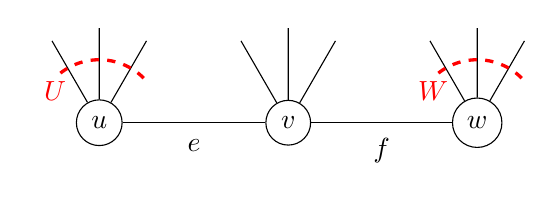
\begin{tikzpicture}[scale=0.8]
\tikzstyle{every node}=[draw,circle]
\foreach \a/\x/\l in {u/-3/U, w/3/W}{
\path  (\x,0) node  (\a) {$\a$};
\path (\a)+(-0.7,0.5) node [color=red,draw=none] (){$\l$};
\foreach \xx in {0,...,2}{
\draw  (\a) -- ++(60+\xx*30: 1.5);}
\draw [dashed,color=red,line width=1.2] (\a)+(45:1) arc (45:135:1);
}
\path  (0,0) node  (v) {$v$};
\draw  (v) -- +(60:1.5) (v) -- +(90:1.5) (v) -- +(120:1.5);
\path (u) edge node [draw=none,below] {$e$} (v);
\path  (w) edge node [draw=none,below] {$f$} (v);
\end{tikzpicture}
\caption{Setting of \cref{lem:crossingcorrelation}} 
\label{fig:crossingcorrelation}
\end{figure}


\begin{lemma}\label{lem:crossingcorrelation}
%\anna{All subscripts $\mu$ not $\nu$.}
Let \hyperlink{tar:G=(V,E,x)}{$G=(V,E,x)$}, and let $\mu$ be a $\lambda$-uniform spanning tree distribution with marginals $x$. 
%Let $u,v,w$ be atoms in a degree cut $S$ and let $\nu$ be $\mu$ conditioned on $u,v,w$ be trees. 
For any pair of edges  $e=(u,v), f=(v,w)$ such that $|\P{e}-1/2|,|\P{f}-1/2|<\eps$ (see \cref{fig:crossingcorrelation}), if $\eps<1/1000$, then
$$\E{W_T | e\not\in T}+\E{U_T | f\not\in T}\leq \E{W_T+U_T}+0.81,$$
where $U=\delta(u)_{-e}$ and $W=\delta(w)_{-f}$.
\end{lemma}
\begin{proof}
All probabilistic statements are with respect to $\nu$ so we drop the subscript.
First, by \cref{lem:wpath}, and negative association we can write,
	\begin{align*}
		\E{W_T |e \not\in T} &\le \E{W_T} + \P{w \in P_{u,v}|e \not\in T}\P{e\in T}\\
		&\le \E{W_T} + \P{w\in P_{u,v}\wedge e\notin T} + 2\eps
		%\E{U_T |f \not\in T} &\le \E{U_T} + \P{f \not\in T \wedge u \in P_{v,w}}.
	\end{align*}
	Note that the lemma only implies  $\E{\delta(w)_T|e\notin T}\leq \E{\delta(w)_T}+\P{w\in P_{u,v}| e\notin T }\P{e\in T}$. To derive the first inequality we also exploit negative association which asserts that the marginal of every edge only goes up under $e\notin T$, so any subset of $\delta(w)$ (in particular $W$) also goes up by at most $\P{e\notin T\wedge w\in P_{u,v}}$.
	Also, the second inequality uses $\P{e\in T} \leq \P{e\notin T} + 2\eps$.
	Using a similar inequality for $U_T$, to prove the lemma it is enough to show that
	\begin{align*}
		\P{w \in P_{u,v} \wedge e \not\in T}
		+\P{u \in P_{v,w} \wedge f \not\in T} \leq 0.806
	\end{align*}
	or that when this inequality fails, a different argument yields the lemma. 
	
	The main observation is that  in any tree it cannot be that both $u$ is on the $v-w$ path and $w$ is on the $u-v$ path. Therefore
	$$\P{u \in P_{v,w} \mid e,f \not\in T} + \P{w \in P_{u,v} \mid e,f \not\in T} \le 1$$
	So, we have
	\begin{align*}
		&\P{e \not\in T \wedge w \in P_{u,v}}+\P{f \not\in T \wedge u \in P_{v,w}} \\
		&\leq 	\P{e,f \not\in T \wedge w \in P_{u,v}}+\P{e\notin T,f\in T}+\PP{\nu}{e,f \not\in T \wedge u \in P_{v,w}}+\P{f\notin T,e\in T}\\
		&\leq  \P{e,f\notin T} + \P{e\notin T,f\in T} + \P{f\notin T, e\in T}\\
		&= 1-\P{e,f\in T}.
	\end{align*}
	It remains to upper bound the RHS. Let $\alpha=\P{f \in T| e\notin T}$. Observe that
	$$ \P{e,f\in T} = \P{f\in T} - \P{f\in T,e\notin T} \geq 1/2-\eps - (1/2+\eps)\alpha.$$
	If $\alpha\leq 0.6$, then $\P{e,f\in T} \geq 0.198$ (using $\eps<0.001$) and the claim follows.
	Otherwise, $\P{f | e\notin T}\geq 0.6$. Similarly, $\P{e | f\notin T}\geq 0.6$. But, by negative association, 
	$$\E{W_T | e\notin T}\leq\E{W_T}+ \P{e} - (\P{f |e\notin T}-\P{f}) \leq  \E{W_T}+2\eps+0.4\leq \E{W_T}+0.405$$ 
	and similarly,   $\E{U_T | f\notin T}\leq  \E{U_T}+0.405$, so the claim follows.
\end{proof}





